\documentclass[12pt]{article}

\usepackage[a4paper,margin=1in]{geometry}
\usepackage{setspace}
\onehalfspacing

\usepackage{amsmath,amssymb,amsthm}
\usepackage{graphicx}
\usepackage{float}
\usepackage{caption}
\usepackage{subcaption}
\usepackage{enumitem}
\usepackage{makecell}
\usepackage{booktabs}
\usepackage{hyperref}

% \begin{figure}[htbp]
%     \centering
%     
\includegraphics[width=0.6\textwidth]{hw1_q2b_surface.png}
%     \caption{Optimal joint density f(p, d)}
%     \label{fig:2b}
% \end{figure}

\title{ECON 5345 Homework 7 Report}
\author{Harlly Zhou}
\date{\today}

\begin{document}

\maketitle

\section*{Question 1}
\begin{enumerate}[label=\alph*.]
    \item The responses and CIs are reported in Figure \ref{fig:1a}. For the ease of comparison, part (b) is plotted on the same figure.Codes in ``hw7\_q1.R''.
    \begin{figure}[htbp]
        \centering
        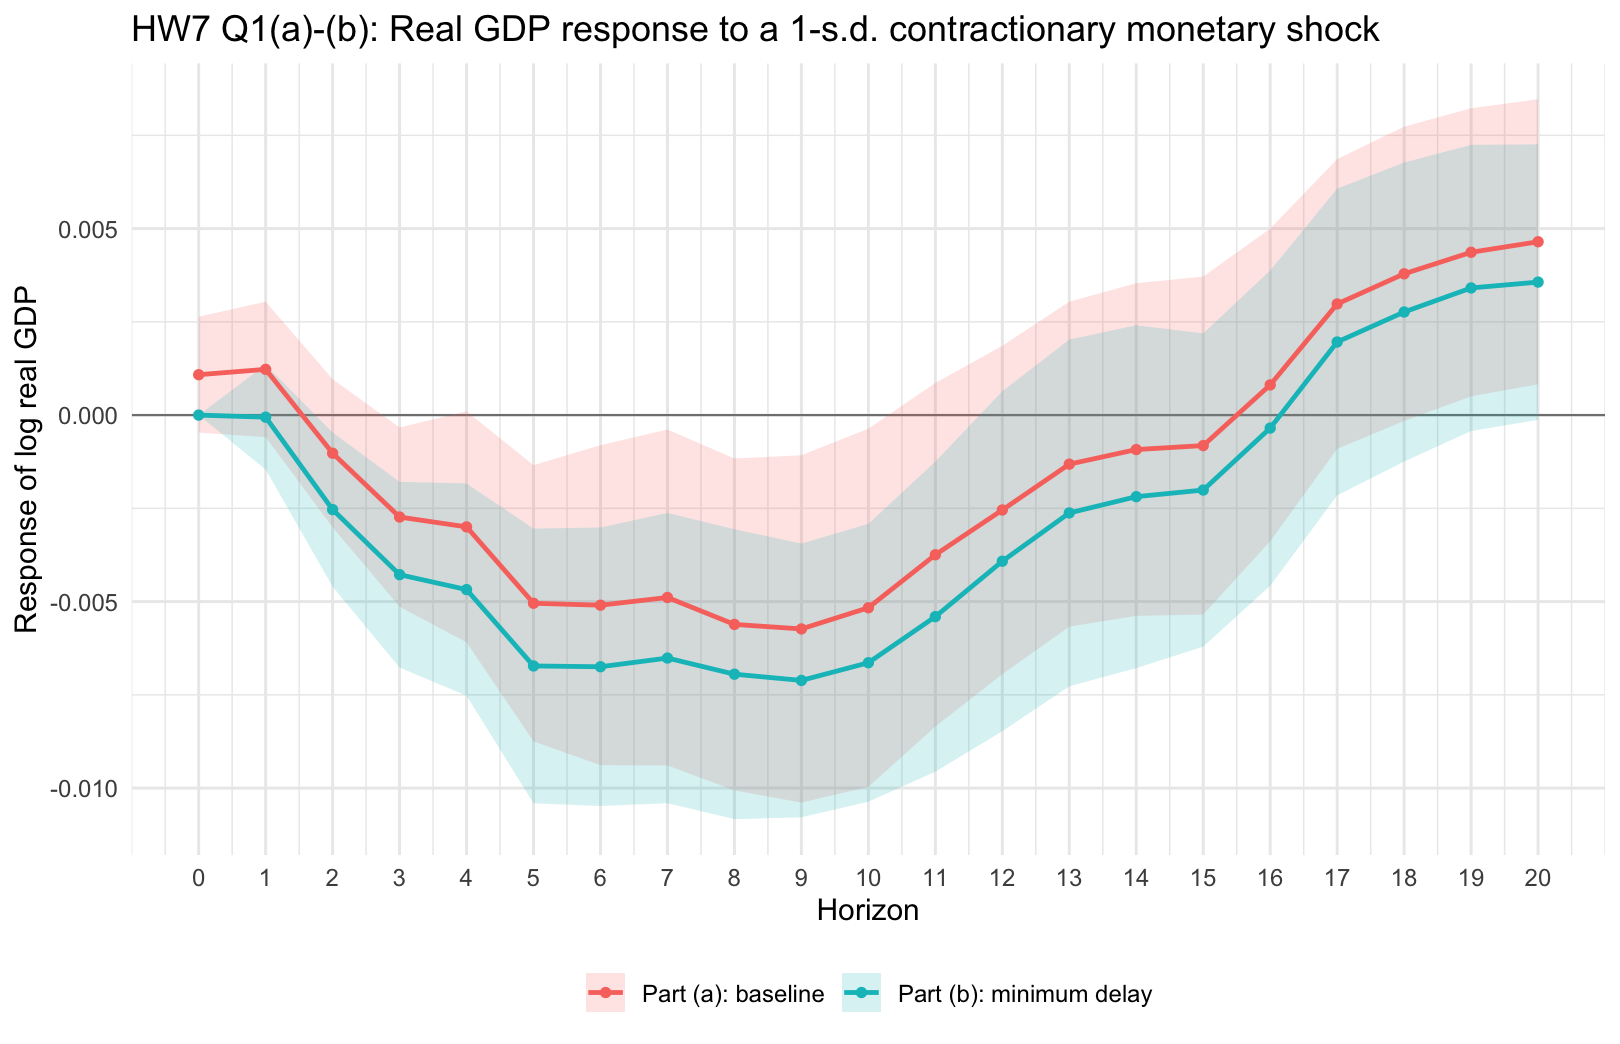
\includegraphics[width=0.6\textwidth]{hw7_q1_ab_gdp_irf.png}
        \caption{GDP IRF and CI}
        \label{fig:1a}
    \end{figure}
    \item See Figure \ref{fig:1a}.
    
    \newpage
    \item The responses and CIs are reported in Figure \ref{fig:1c}. Codes in ``hw7\_q1.R''.
    \begin{figure}[htbp]
        \centering
        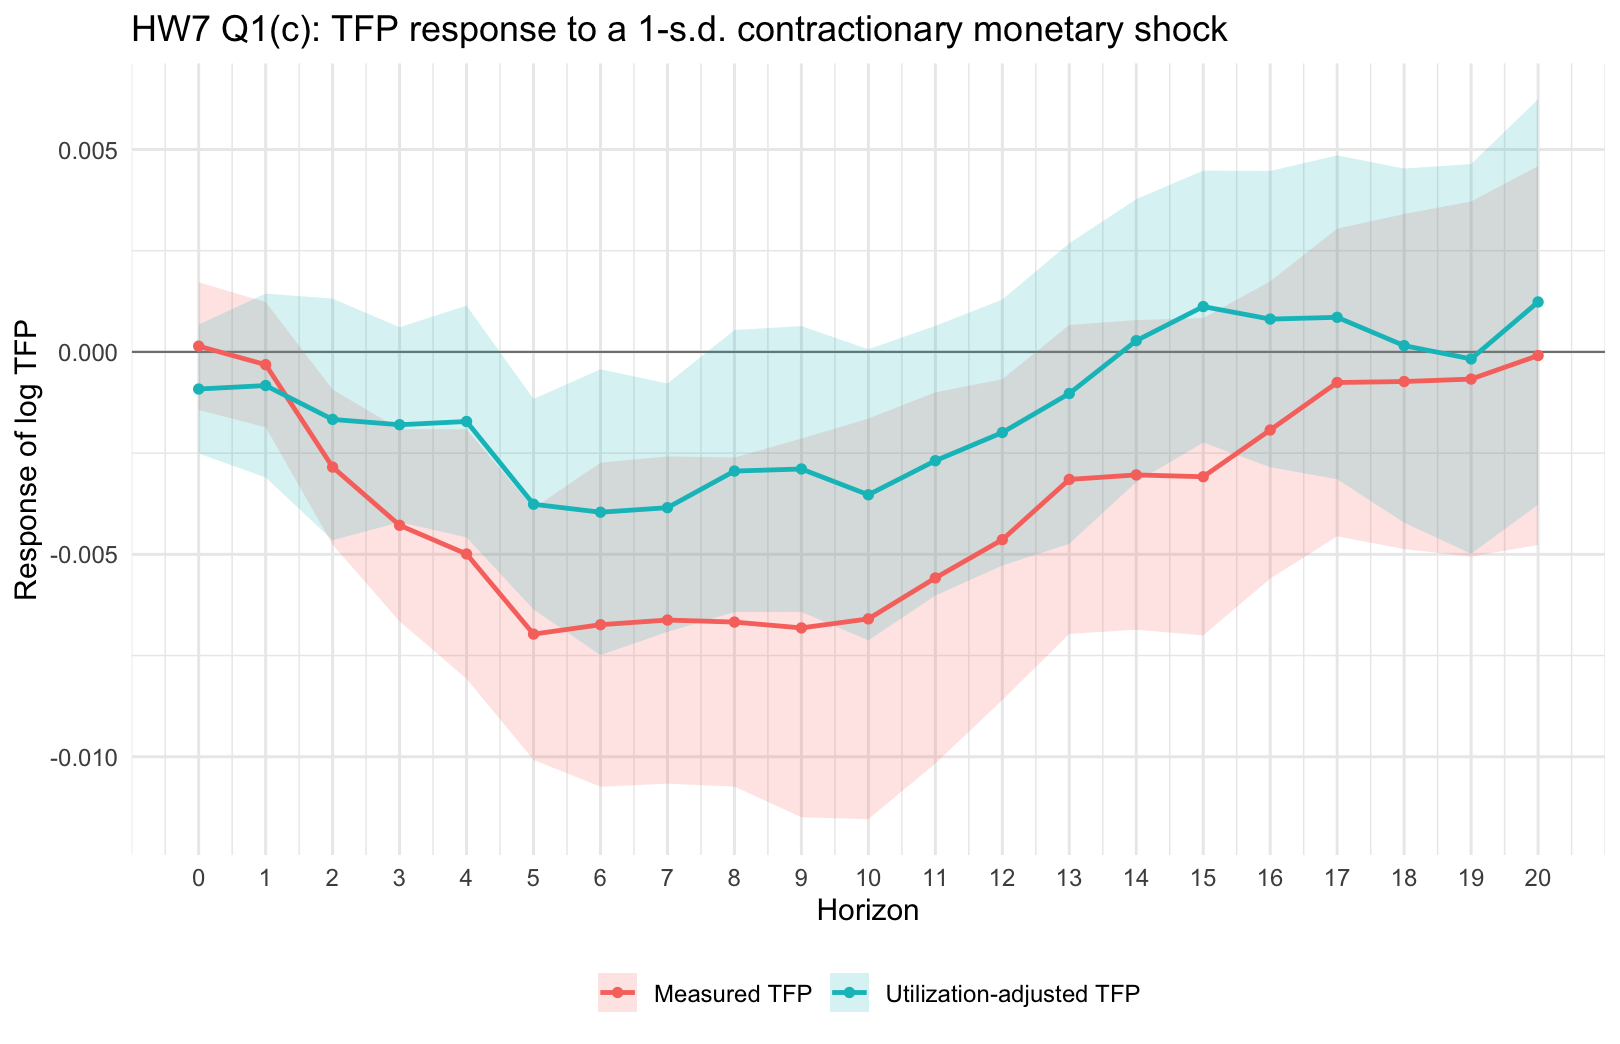
\includegraphics[width=0.6\textwidth]{hw7_q1_c_tfp_irf.png}
        \caption{TFP IRF and CI}
        \label{fig:1c}
    \end{figure}

    The measured TFP response has a delayed but statistically significant reponse to the monetary policy shock after around 2 quarters. The utilization-adjusted TFP has alomst no staistically significant response to the monetary policy shock. Since TFP should not endogenously respond to monetary policy shock, this suggests that the utilization-adjusted TFP is a better measure of TFP.
\end{enumerate}

\newpage
\section*{Question 2}
\begin{enumerate}[label=\alph*.]
    \item We have $z_t = \begin{pmatrix}
        y_t \\
        y_{t-1} \\
        \varepsilon_t \\
        \varepsilon_{t-1}
    \end{pmatrix}$. Then we can write
    \begin{align*}
        z_t = \begin{pmatrix}
            y_t \\
            y_{t-1} \\
            \varepsilon_t \\
            \varepsilon_{t-1}
        \end{pmatrix}
        = \begin{pmatrix}
            \alpha & 0 & \theta & 0 \\
            1 & 0 & 0 & 0 \\
            0 & 0 & 0 & 0 \\
            0 & 0 & 1 & 0
        \end{pmatrix}
        \begin{pmatrix}
            y_{t-1} \\
            y_{t-2} \\
            \varepsilon_{t-1} \\
            \varepsilon_{t-2}
        \end{pmatrix}
        + \begin{pmatrix}
            1 \\
            0 \\ 
            1 \\
            0
        \end{pmatrix}
        \varepsilon_t
    \end{align*}
    and $y_t = (\, 1 \quad 0 \quad 0 \quad 0\, ) z_t$.

    \item The following table reports the estimates:
    \begin{table}[htbp]
        \centering
        \begin{tabular}{lccccccc}
            \toprule
            $T$ & $\hat{\alpha}$ & $\hat{\theta}$ &  $\hat{\sigma}^2$ & se($\hat{\alpha}$) & se($\hat{\theta}$) & se($\hat{\sigma}$) & LogLik \\
            \midrule
            50  & 0.5895 & 0.4642 & 2.1740 & 0.1316 & 0.1523 & 0.1510 & -101.7544 \\
            100 & 0.7960 & 0.4234 & 2.5275 & 0.0693 & 0.1106 & 0.1137 & -199.3829 \\
            500 & 0.7835 & 0.3898 & 3.0852 & 0.0306 & 0.0466 & 0.0557 & -1001.9500 \\
            \bottomrule
        \end{tabular}
        \caption{Estimation results for different sample sizes}
    \end{table}

    \newpage
    \item I first present the statistics for $\sigma^2$ because in HR and MoM I did not report them.
    \begin{table}[htbp]
        \centering
        \begin{tabular}{lrrrr}
        \toprule
        $T$ & Bias & Variance & MSE & SD \\
        \midrule
        50  & -0.0314 & 0.3892 & 0.3898 & 0.624 \\
        100 & -0.0469 & 0.1802 & 0.1822 & 0.425 \\
        500 & -0.0186 & 0.0331 & 0.0334 & 0.182 \\
        \bottomrule
        \end{tabular}
        \caption{Estimation performance for $\sigma^2$ (Kalman Filter).}
        \end{table}
    
    
        The comparison of the estimates are reported in Table \ref{tab:2c}. For $\alpha$ estimation, the Kalman filter has better performance especially when the sample size is small. For $\theta$ estimation, the Kalman filter has better performance when the sample size is large. 
    \begin{table}[htbp]
        \centering
        \begin{tabular}{lrrrrr}
        \toprule
        $T$ & Parameter & Bias & Variance & MSE & SD \\
        \midrule
        
        \multicolumn{6}{c}{\textbf{Kalman Filter}} \\
        \midrule
        50  & $\alpha$ &  0.0072 & 0.0109 & 0.0109 & 0.104 \\
        50  & $\theta$ & -0.1175 & 0.0654 & 0.0792 & 0.256 \\
        
        100 & $\alpha$ & -0.0011 & 0.0052 & 0.0052 & 0.072 \\
        100 & $\theta$ & -0.0479 & 0.0240 & 0.0263 & 0.155 \\
        
        500 & $\alpha$ & -0.0026 & 0.0009 & 0.0009 & 0.030 \\
        500 & $\theta$ & -0.0011 & 0.0021 & 0.0021 & 0.046 \\
        
        \midrule
        \multicolumn{6}{c}{\textbf{HR}} \\
        \midrule
        50  & $\alpha$ & -0.09 & -- & 0.02 & 0.13 \\
        50  & $\theta$ &  0.01 & -- & 0.02 & 0.15 \\
        
        100 & $\alpha$ & -0.04 & -- & 0.01 & 0.08 \\
        100 & $\theta$ & -0.00 & -- & 0.01 & 0.11 \\
        
        500 & $\alpha$ & -0.01 & -- & 0.00 & 0.03 \\
        500 & $\theta$ & -0.00 & -- & 0.00 & 0.05 \\
        
        \midrule
        \multicolumn{6}{c}{\textbf{MoM}} \\
        \midrule
        50  & $\alpha$ & -0.05 & -- & 0.02 & 0.12 \\
        50  & $\theta$ &  0.06 & -- & 0.06 & 0.24 \\
        
        100 & $\alpha$ & -0.02 & -- & 0.01 & 0.08 \\
        100 & $\theta$ &  0.04 & -- & 0.04 & 0.19 \\
        
        500 & $\alpha$ & -0.01 & -- & 0.00 & 0.03 \\
        500 & $\theta$ &  0.01 & -- & 0.00 & 0.07 \\
        
        \bottomrule
        \end{tabular}
        \caption{Comparison of estimation performance for $\alpha$ and $\theta$.}
        \label{tab:2c}
        \end{table}
\end{enumerate}




\end{document}